\section{Auswertung}

\subsection{Bestimmung der Zeitkonstante eines RC-Glieds}

Wir verwenden die in Aufgabenteil 1 gemessenen Halbwertszeiten, um die Zeitkonstante nach Gleichung \eqref{eq:zeitkonst} zu berechnen. Den theoretischen Wert der Zeitkonstante ermitteln wir anhand der Formel $\tau = RC$ mit dem Widerstand $R$ und der Kapazität $C$. Die resultate der Berechnungen für alle vier Konfigurationen der RC-Schaltung sind \tabref{tab:a1_zeitkonst} zu entnehmen.

\begin{table}[h]
  \centering
  \begin{tabular}{| c | c | c | c | c | c |}
      \hline
      $C\ [\si{\nano\farad}]$ & $R\ [\si{\kilo\ohm}]$ & $f\ [\si{\hertz}]$ & $\tau_{\text{theo}}\  [\si{\second}]$ & $\tau_{\text{exp}}\ [\si{\second}]$ & Abw. \\
      \hline
      $470 \pm 47$ & $1.00 \pm 0.05$ & $165 \pm 1$ & $(47 \pm 6) \times 10^{-5}$ & $(43 \pm 15) \times 10^{-5}$ & $0.25\sigma$ \\
      \hline
      $4.70 \pm 0.47$ & $10.00 \pm 0.50$ & $165 \pm 1$ & $(4.7 \pm 0.6) \times 10^{-5}$ & $(6.49 \pm 0.15) \times 10^{-5}$ & $3.29\sigma$ \\
      \hline
      $47.00 \pm 4.70$ & $1.00 \pm 0.05$ & $165 \pm 1$ & $(4.7 \pm 0.6) \times 10^{-5}$ & $(4.91 \pm 0.15) \times 10^{-5}$ & $0.38\sigma$ \\
      \hline
  \end{tabular}
  \caption{Messwerte und berechnete Größen}
  \label{tab:a1_zeitkonst}
\end{table}

\abbref{fig:aufgabe1_rc_signalverlauf} zeigt exemplarisch den Spannungsverlauf für die letzte angegebene Schaltungskonfiguration. 


\begin{figure}[H]
  \centering
  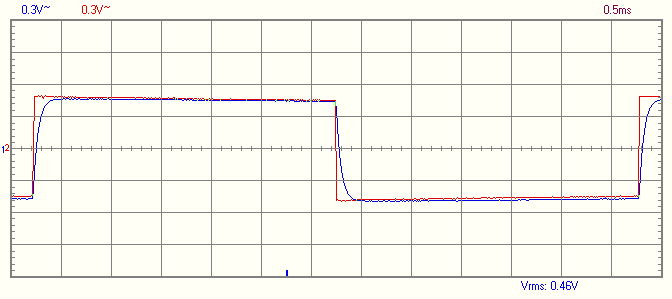
\includegraphics[width=.8\textwidth]{files/aufgabe1_rc_signalverlauf.png}
  \caption{Spannungsverlauf am Oszilloskop des RC-Glieds für $C = 47\si{\nano\farad}$, $R = 1 \si{\kilo\ohm}$. In Rot dargestellt die Eingangsspannung $U_E$, in Blau die Ausgangsspannung $U_C$, abgenommen über den Kondensator.}
  \label{fig:aufgabe1_rc_signalverlauf}
\end{figure}

\subsection{RC-Glied als Integrator und Differentiator}

Wie bereits dem Versuchsprotokoll zu entnehmen können wir beim Aufbau der RC-Schaltung als Integrator beobachten, dass sich das Ausgangssignal bei Erhöhung des Widerstandes immer stärker dem Integral des Eingangssignals annähert. So formt ein eingehendes Rechteckssignal eine Dreiecksfunktion als Ausgangssignal, aus einem eingehenden Dreieckssignal ergibt sich ein Sinussignal, wie in \abbref{fig:aufgabe2_integral_dreieck} zu sehen.

\begin{figure}[H]
  \centering
  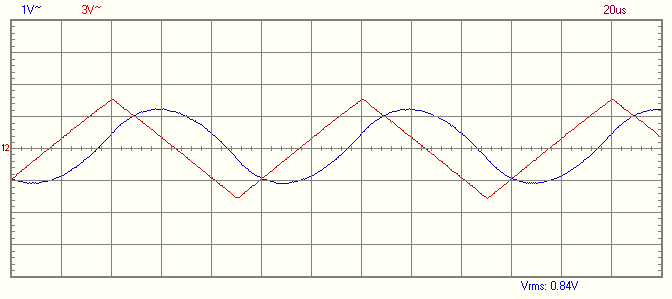
\includegraphics[width=.8\textwidth]{files/aufgabe2_integral_dreieck.png}
  \caption{Spannungsverlauf beim Betrieb der RC-Schaltung als Integrator. In Rot dargestellt die dreiecksförmige Eingangsspannung $U_E$, in Blau die Ausgangsspannung $U_C$, abgenommen über den Kondensator.}
  \label{fig:aufgabe2_integral_dreieck}
\end{figure}

Ähnliche Beobachtungen können wir beim Betrieb des RC-Glieds als Differentiator machen. Bei Justierung des Widerstandes ergibt sich hierbei beispielsweise aus einem eingehenden Dreieckssignal ein ausgehendes Rechteckssignal, siehe \abbref{fig:aufgabe2_differentiator_dreieck}. Geben wir durch den Funktiongenerator ein Signal in der Form einer Gauß'schen Normalverteilung ein, so ergibt sich auch hiervon die entsprechende Ableitung, zu sehen in \abbref{fig:aufgabe2_differentiator_gauss}.


\begin{figure}[H]
  \centering
  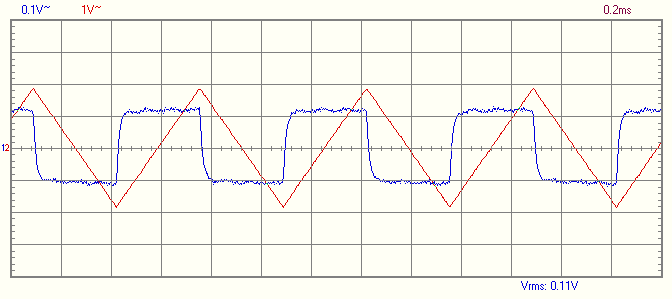
\includegraphics[width=.8\textwidth]{files/aufgabe2_differentiator_dreieck.png}
  \caption{Spannungsverlauf beim Betrieb der RC-Schaltung als Differentiator. In Rot dargestellt die dreiecksförmige Eingangsspannung $U_E$, in Blau die Ausgangsspannung $U_R$, abgenommen über den Widerstand.}
  \label{fig:aufgabe2_differentiator_dreieck}
\end{figure}

\begin{figure}[H]
  \centering
  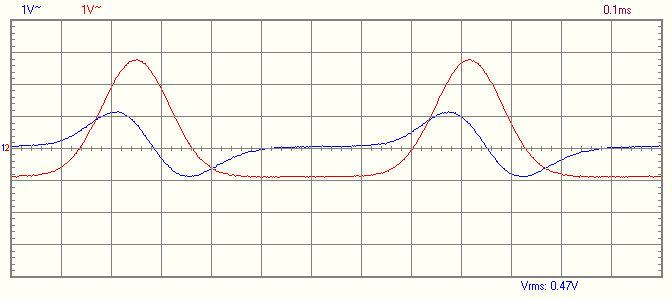
\includegraphics[width=.8\textwidth]{files/aufgabe2_differentiator_gauss.png}
  \caption{Spannungsverlauf beim Betrieb der RC-Schaltung als Differentiator. In Rot dargestellt die Eingangsspannung $U_E$, in Blau die Ausgangsspannung $U_R$, abgenommen über den Widerstand.}
  \label{fig:aufgabe2_differentiator_gauss}
\end{figure}


\subsection{Frequenz- und Phasengang eines RC-Glied}

In diesem Teil der Auswertung bestimmen wir aus dem aufgezeichneten Frequenzgängen eines Tief- und Hochpassfilters die Grenzfrequenz bestimmen. Wie in den theoretischen Grundlagen erklärt, ist die Grenzfrequenz der Filterschaltung dadurch zu erkennen, dass bei ihr die Amplitude um den Faktor $\flatfrac{1}{\sqrt{2}}$ abgefallen ist. Mit der \textit{Curser}-Funktion des Oszilloskops können wir damit eine Grenzfrequenz von $(9.46 \pm 0.02)\si{\hertz}$ für den Tiefpassfilter und eine Grenzfrequenz von $(3.31 \pm 0.02) \si{\hertz}$ für den Hochpassfilter ablesen. Die untenstehenden Abbildungen zeigen noch einmal die Frequenzgänge des Tiefpassfilters (\ref{fig:aufgabe3_tiefpass}) und Hochpassfilters (\ref{fig:aufgabe3_hochpass}), jeweils mit dem Cursor an der Grenzfrequenz.


\begin{figure}[H]
  \centering
  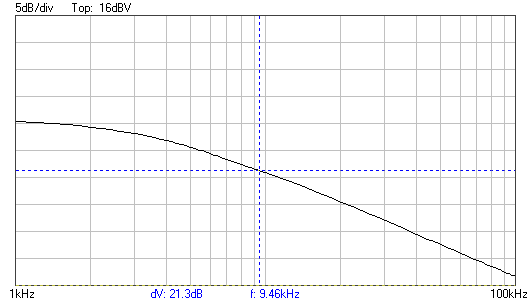
\includegraphics[width=.8\textwidth]{files/aufgabe3_tiefpass.png}
  \caption{Frequenzgang des Tiefpassfilters mit Cursor bei Grenzfrequenz}
  \label{fig:aufgabe3_tiefpass}
\end{figure}

\begin{figure}[H]
  \centering
  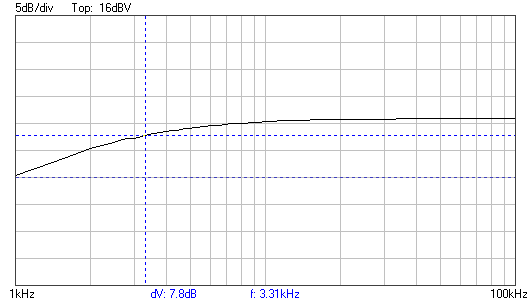
\includegraphics[width=.8\textwidth]{files/aufgabe3_hochpass.png}
  \caption{Frequenzgang des Hochpassfilters mit Cursor bei Grenzfrequenz}
  \label{fig:aufgabe3_hochpass}
\end{figure}

Neben der Aufzeichnung des Frequenzgangs haben wir für den Hochpassfilter zusätzlich den Phasengang manuell vermessen. Die Phase $\varphi$ ist in \abbref{fig:phaseshift_hp_fit} über der Frequenz aufgetragen. Die Grenzfrequenz bestimmen wir nun durch Ablesen Frequenz bei einer Phase von $45\si{\degree}$. Die Phase zeigt, abhängig von der Frequenz, einen logarithmisch abfallenden Verlauf auf. Um den Wert bei $45\si{\degree}$ interpolieren zu können fitten wir eine abfallende Exponentialfunktion der Form
\begin{align}
  f(x; A,\lambda,c) = A \cdot \e{- \lambda x} + c
\end{align}
an die Datenpunkte an. Die optimierten Werte der Parameter sind ebenfalls der \abbref{fig:phaseshift_hp_fit} zu entnehmen.


\begin{figure}[H]
  \centering
  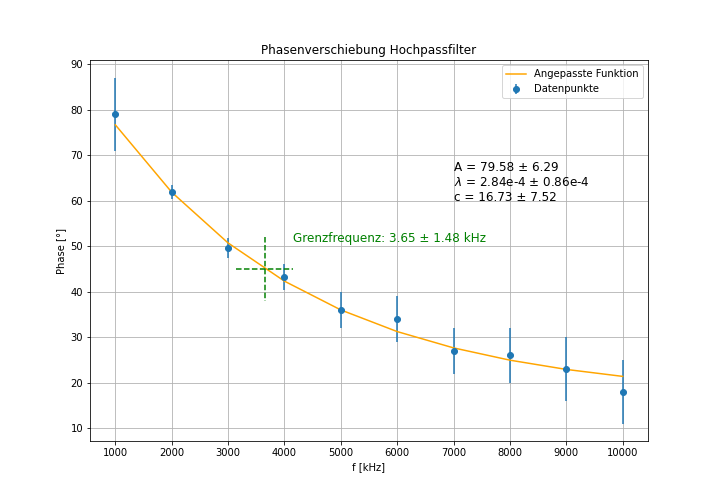
\includegraphics[width=.8\textwidth]{files/phaseshift_hp_fit.png}
  \caption{Phasengang des Hochpassfilters mit exponentiellem Fit und Grenzfrequenz bei $45\si{\degree}$.}
  \label{fig:phaseshift_hp_fit}
\end{figure}


Durch elementares Umformen bestimmen wir die Umkehrfunktion von $f$, um damit die Grenzfrequenz berechnen zu können. Für diese gilt
\begin{align}
  f^{-1}(\varphi; A, \lambda, c) = - \frac{1}{\lambda} \ln(\frac{\varphi - c}{A}) = f_{\mathrm{Grenz}}.
\end{align}
Nach der gauß'schen Fehlerfortpflanzung gilt für der Fehler des damit berechneten Wertes
\begin{align}
  \Delta f_{\mathrm{Grenz}} = \sqrt{\qty(\frac{1}{\lambda A} \ln(\frac{\varphi - c}{A}) \cdot \Delta A)^{2} + \qty(\frac{1}{\lambda^2} \ln(\frac{\varphi - c}{A}) \cdot \Delta \lambda)^{2} + \qty(\frac{1}{\lambda(\varphi - c)} \cdot \Delta c)^{2}}.
\end{align}

Damit können wir aus der Funktion eine Grenzfrequenz von
\begin{align}
  f_{\mathrm{Grenz}} = (3.65 \pm 1.48) \si{\kilo\hertz}
\end{align}
interpolieren. Diese ist ebenfalls in Grün in \abbref{fig:phaseshift_hp_fit} markiert. Von der zuvor vermessenen Grenzfrequenz weicht diese um etwa $2.47\sigma$ ab, was innerhalb des $3\sigma$-Bereichs noch als eine nicht signifikante Abweichung angesehen werden kann.

\subsection{Frequenzgang eines Serienschwingkreises}

Für diesen Aufgabenteil betrachten wir erstmals einen Serienschwingkreis, also eine Schaltung bestehend aus Kondensator, Widerstand und Spule. Im ersten Schritt möchten wir die Induktivität der verbauten Spule berechnen, dazu ziehen wir \eqref{eq:rlc_omega_r} hinzu und stellen diese um nach
\begin{align}
  L &= \frac{1}{\omega_R^2 C}
\end{align}
mit der Kapazität $C$, sowie gemessenen Resonanzfrequenz $\omega_R$, welche wir zuvor durch den Faktor $2\pi$ noch in eine Kreisfrequenz umrechnen. In der Durchführung haben wir die Messungen für drei unterschiedliche Widerstände durchgeführt, also drei verschiedene Resonanzfrequenzen gemessen. Für die drei Frequenzen berechnen wir jeweils eine Induktivität und nehmen davon den Mittelwert von
\begin{align}
  L = (3.63 \pm 2.11) \cdot 10^{-2} \si{\henry}
\end{align}
als Wert für die Induktivität der Spule.

Als Nächstes betrachten wir die Verluste, welche in der Spule durch ihren eigenen ohmschen Widerstand, magnetische Verluste des Spulenkerns, sowie den Skineffekt entstehen. Um diese Verluste zu quantifizieren, nehmen wir die Existenz eines weiteren Verlustwiderstandes $R_V$ in der Schaltung an. \eqref{eq:rlc_bandbreite} stellt einen Zusammenhang zwischen dem Gesamtwiderstand und der Bandbreite der RLC-Schaltung her, welchen wir entsprechend umstellen zu
\begin{align}
  R + R_V = \Delta \omega \cdot L.
\end{align}

Wie im Theorieteil beschrieben stellt das RLC-Glied im Resonanzfall bei $\omega_R$ einen Kurzschluss dar, da die Impedanz des LC-Gliedes verschwindet. Für das Verhältnis von Ein- und Ausgangsspannung, letztere abgenommen am Widerstand $R$, ergibt sich somit der einfache Zusammenhang
\begin{align}
  U_A = \frac{R}{R + R_V} U_E
\end{align}
und somit durch
\begin{align}
  R + R_V &= R \frac{U_E}{U_A}
\end{align}
eine weitere Formel, um den Gesamtwiderstand zu berechnen. Die folgende Tabelle zeigt nun die in den drei Messgängen aufgezeichneten Werte der Ein- und Ausgangsspannung $U_E$ und $U_A$, der Resonanzfrequenz $\omega_R$, sowie der Bandbreite $\Delta \omega$. Als Induktivität verwenden wir den zuvor berechneten Mittelwert. Weiter enthält die Tabelle die berechneten Werte für $R + R_V$, den verwendeten Widerstand, sowie deren Differenz, also die Verlustleistung $R_V$.

\begin{table}[H]
  \centering
  \begin{tabular}{|c|c|c|c|c|}
    \hline
    \multicolumn{2}{|c|}{$R\,[\si{\ohm}]$} & $1000 \pm 50$ & $220 \pm 11$ & $47.0 \pm 2.4$ \\
    \hline
    \multicolumn{2}{|c|}{$U_E\,[\si{\volt}]$} & $0.661 \pm 0.001$ & $0.650 \pm 0.001$ & $0.627 \pm 0.001$ \\
    \hline
    \multicolumn{2}{|c|}{$U_A\,[\si{\volt}]$} & $0.640 \pm 0.020$ & $0.530 \pm 0.020$ & $0.270 \pm 0.020$ \\
    \hline
    \multicolumn{2}{|c|}{$\Delta \omega\,[\si{\per\second} \cdot 10^3]$} & $30.91 \pm 0.19$ & $8.11 \pm 0.19$ & $3.52 \pm 0.19$ \\
    \hline
    \hline
    \multirow{2}{*}{Aus Bandbreite} & $R + R_V\,[\si{\ohm}]$ & $1123 \pm 650$ & $294 \pm 171$ & $128 \pm 75$ \\
    \cline{2-5}
    & $R_V\,[\si{\ohm}]$ & $123 \pm 652$ & $74 \pm 171$ & $80 \pm 75$ \\
    \hline
    \hline
    \multirow{2}{*}{Aus Amplituden} & $R + R_V\,[\si{\ohm}]$  & $1033 \pm 61$ & $270 \pm 17$ & $109 \pm 10$ \\
    \cline{2-5}
    & $R_V\,[\si{\ohm}]$ & $33 \pm 79$ & $49.811 \pm 21$ & $62.144 \pm 11$ \\
    \hline
  \end{tabular}
\end{table}